\documentclass[aspectratio=169,fleqn,xcolor={dvipsnames},handout]{beamer}

\usetheme[pageofpages=of]{hubln}
% dette dokumentet er hoveddokumentet og må kompileres
% resten skjer i Preamble.tex

\usepackage[utf8]{inputenc}
\usepackage[T1]{fontenc}
\usepackage[norsk]{babel}
\usepackage{tabularx}
\usepackage{hhline}
\usepackage{array}
\usepackage{tikz}
\usepackage{tikz-cd}
\usepackage{amsmath}
\usepackage{amssymb}
\usepackage{mathtools}
\usepackage{cancel}
\usepackage{multirow}
\usepackage{comment}
\usepackage{minted,xcolor}
\usepackage{caption}
\usepackage{subcaption}
\usetikzlibrary{cd}
\usetikzlibrary{babel}
\usepackage{relsize}
\usepackage{amssymb}
\usepackage{csquotes}
\usemintedstyle{monokai} %vs
%\definecolor{bg}{HTML}{282828}
\definecolor{bg}{RGB}{40, 40, 40}
\setminted{bgcolor=black,frame=lines,
               framesep=2mm}
\usefonttheme{professionalfonts}
\setbeamercovered{invisible}
\hfuzz=8.64pt % Antioverfullbox-inator

\setbeamercolor{block body alerted}{bg=alerted text.fg!10}
\setbeamercolor{block title alerted}{bg=alerted text.fg!20}
\setbeamercolor{block body}{bg=structure!10}
\setbeamercolor{block title}{bg=structure!20}
\setbeamercolor{block body example}{bg=green!10}
\setbeamercolor{block title example}{bg=green!20}
\setbeamertemplate{blocks}[rounded][shadow]


\tikzset{onslide/.code args={<#1>#2}{% from https://tex.stackexchange.com/a/6155/263192
  \only<#1>{\pgfkeysalso{#2}}
}}

\newcommand{\newLine}{%
  \hfill\break
}

%\newcommand{\comment}[1]{}
\tikzset{vertex/.style={draw, circle, inner sep=1mm}}
\newcommand{\incomplete}[3][1.5cm]{\begin{tikzpicture}
\foreach \n in {1,...,#2}{\node[vertex]at({90-360/#2*(\n-1)}:#1)(\n){\n};}
\foreach \v/\w in {#3}{\draw(\v)--(\w);}
\end{tikzpicture}}
\tikzset{properties/.style={orange, ultra thick}}
\tikzset{propertiesRed/.style={red, ultra thick}}
\tikzset{propertiesBlue/.style={blue, ultra thick}}
\tikzset{propertiesGrey/.style={gray, ultra thick}}

\usepackage{mathtools}
\DeclarePairedDelimiter\ceil{\lceil}{\rceil}
\DeclarePairedDelimiter\floor{\lfloor}{\rfloor}

% Hier die Daten zur Präsentation eintragen
\author[ls]{Steinar Simonnes og Lukas Schramm}
\title[sgp]{Kræsjkurs MNF130}
\institute{Institutt for informatikk \\ Universitetet i Bergen}
\date[12.05.22]{12 Mai 2022}

\begin{document}
  % Innholdet til selveste presentasjon

% Titel page
\begin{frame}[t,plain]
    \titlepage
\end{frame}

% table of contents (skjer automatisk)
\section{Innføring}
\subsection*{Agenda}
\begin{frame}
    %\tableofcontents
    \begin{columns}[t]
        \begin{column}{.5\textwidth}
            \tableofcontents[sections={1-6}]
        \end{column}
        \begin{column}{.5\textwidth}
            \tableofcontents[sections={7-}]
        \end{column}
    \end{columns}
\end{frame}

\subsection*{Download PDFen}
\begin{frame}{Last meg ned}
    \begin{figure}
        \centering
        
\includegraphics[height = 4.9cm]{images/downloadqr.png}
        \caption{https://tinyurl.com/mnf130v22}
        \label{fig:qrcode}
    \end{figure}
\end{frame}

%%\section*{LaTeX Steinar}
\subsection*{Teamer}
\begin{frame}{Temaer}
\begin{itemize}
    \item Hver section er noe som vises på Table of contents og øverst som tema
    \item Hver subsection vises i andre rad i denn blåe boksen
    \item bruk stjerne for subsection dersom den ikke skal inn i table of contents
    \item Hver slide skrives inn i \textit{itemize environment}
\end{itemize}
\end{frame}

\subsection*{Eksempel for tabeller}
\begin{frame}{Eksempel}
%en tabell skrives inn i tabular environment
%\begin{center}
\begin{tabular}{l|l|l|l|l}
 StudentNr & Name & Address & KursNr & KursName \\\hline
 580 & Ola NordmaNN & 5075 Bergen Fv 14 & INF237 & Algorithm Engineering\\
 580 & Ola NordmaNN & 5075 Bergen Fv 14 & INF273 & Meta Heuristikker\\
 580 & Ola NordmaNN & 5075 Bergen Fv 14 & INF227 & Logik\\
 256 & Max MustermaNN & 5055 Bergen Lv 85 & INF237 & Algorithm Engineering\\
\end{tabular}
\\[5mm] %avstand fra tabellen
en tabell skrives inn i tabular environment\\
før eller etter tabellen kan det står andre ting, husk å sette avstanden
%\end{center}
\end{frame}

\begin{frame}{Hvordan ha flere tabeller samtidige?}
% svaret er hvill og vfill
\begin{tabular}{l|l|l}
 StudentNr & Name & Address\\\hline
 580 & Ola NordmaNN & 5075 Bergen Fv 14\\
 256 & Max MustermaNN & 5055 Bergen Lv 85\\
\end{tabular}
\vfill
\begin{tabular}{l|l}
KursNr & KursName \\\hline
INF237 & Algorithm Engineering\\
INF273 & Meta Heuristikker\\
INF227 & Logikk\\
\end{tabular}
\hfill
\begin{tabular}{l|l}
 StudentNr & KursNr\\\hline
 580 & INF237\\
 580 & INF273\\
 580 & INF227\\
 256 & INF237\\
\end{tabular}
\end{frame}

% etter hvert tema har vi et bilde av Guillaume som spør noe
\subsection*{Spørretid}
\begin{frame}{Spørsmål?}
    \begin{figure}
        \centering
        \includegraphics[height = 4.9cm]{images/guillaume9.jpg}
        \caption{Guillaume foran Tvindefossen}
        \label{fig:guillaume9}
    \end{figure}
\end{frame}

%=================================
\subsection*{Hva Steinar skulle vite}
\begin{frame}{LaTeX informasjoner for Steinar}
\begin{itemize}
    \item En frame er teknisk sett ikke det samme som en side. Vi kan innstille at ting etter hvert dykker opp på en slide, da består en side av flere frames, altså forskjellige ting som vises
    \item Den neste sliden forklarer det
\end{itemize}
\end{frame}

\subsection*{Synlighet Lister}
\begin{frame}{Itemize: Automatisk oppdykking av neste punkter}
%% [<+->] en liste dykker opp med et element hver
%% [<+(2)->] skrittlengde er to
\begin{itemize}[<+->]
    \item Itemize funker som i LaTeX
    \item Kommandoen oppe gjør at hver element dykker opp på neste slide
    \item Alt som funker som lister kan dette automatisk
\end{itemize}

\end{frame}

%% <1-> setter på hvilke sub-frames noe skal være synnlig
\begin{frame}{Itemize: Eksplisit synnlighet}
\begin{itemize}
    \item<1-> Dette punktet er synlig fra frame 1 til slutten
    \item<2-> Dette punktet er synlig fra frame 2 til slutten
    \item<2-3> Den også
    \item<3-> Den dykker opp som tredje
    \item<4-> Da er det noe som har forsvunnet!
\end{itemize}

\end{frame}
% \pause Det samme kan gjøres med pause
\begin{frame}{Itemize: Pause}
\begin{itemize}
    \item Det samme kan gjøres med \texttt{pause}
    \item Alt dykker opp til neste pause kommando
    \pause
    \item Også kommer det neste delen til slutten eller neste pausekommandoen
\end{itemize}

\end{frame}

\subsection*{En ting til med pause}
%% Pause kan også brukes for alt på en slide
\begin{frame}{Pause med tekst}
Pause kan også brukes innenfor en stor tekst.\pause~Og alt mulig annet.\pause~Tildesymbolen trengs fordi \LaTeX ellers mangler en space
\end{frame}
%
\begin{frame}{Resten}
Resten er ting som er skrevet på tysk som Lukas var for lat å oversette. Det er mange fine ting blant det, men det kan vi se på senere
\end{frame}

%% Der Visible-Befehl sagt an, auf welchen Folien etwas sichtbar sein soll (analog zu <a-b>)
%\begin{frame}{Der Visible-Befehl}
%Auch der von-bis-Befehl hat für beliebige Sachen ein Pendant. Man kann mit dem \texttt{Visible}-Befehl und geschwungenen Klammern einen Bereich umrahmen, der nur von Teil-Seite x bis y sichtbar sein wird.
%
%\newLine % Der NewLine-Befehl wurde in der Präambel definiert und ist kein LaTeX-Standard. Er führt zu einem angenehmen Zeilenumbruch, der für Zentrierung der Inhalte einer Folie führt
%\visible<2-3>{
% $ G := (V, E)$ with $V$ a set of vertices and $E := \{ (a, b)$ and $(b, a)$ with $a, b \in V $ and $ a \neq b \} $
%
%}
%    
%\visible<3-3>{
%  \newLine
%  $ G = (\{1, 2, 3, 4, 5, 6\}, \{(1, 2), (2, 1),
%      (1, 3), (3, 1),
%      (1, 4), (4, 1), 
%      (2, 4), (4, 2), $ \\
%  \quad\quad $ (2, 5), (5, 2),
%      (2, 6), (6, 2),
%      (3, 4), (4, 3),
%      (3, 6), (6, 3),
%      (5, 6), (6, 5)\}) $
%}
%
%\visible<4>{
%  \begin{center}
%    Ich lasse nun all den Mathekram verschwinden
%  \end{center}
%}
%\end{frame}
%
%
%% Der Only-Befehl funktioniert ähnlich wie visible, gibt jedoch den Platz wieder an das nächste Element zurück
%\begin{frame}{Der Only-Befehl}
%Der Only-Befehl funktioniert wie Visible, aber gibt den Platz wieder frei\\
%\begin{center}
%  \begin{tabular}{cccccc}
%    $ \begin{tabular}{c}1: \\2: \\3: \\4: \\5: \end{tabular} $ &
%    $ \begin{bmatrix}-1.28078 \\0.280776 \\-1 \\-1.28078 \\2.28078 \end{bmatrix} $ &
%    $\rightarrow$ &
%    $ \begin{bmatrix}-1 \\1 \\-1 \\-1 \\1 \end{bmatrix} $ &
%    \visible<2>{$\rightarrow$} &
%    \visible<2>{\noindent\parbox[c]{2.5cm}{ $V_1 = \{1,3,4\}\\V_2 = \{2,5,6\}$}}
%  \end{tabular}\\
%  % Anmerkung: Die Mathematik dieser Folie ist nicht korrekt und dient Anschauungszwecken
%  
%  \only<1>{% Graph 1 ist auf der ersten Folie sichtbar
%    \myGraph
%  }
%  \only<2>{% Graph 2 ist auf der nächsten Folie an seiner Stelle sichtbar
%    \myGraphCorrect
%  }
%\end{center}
%\end{frame}
%
%\section{Sonstiges}
%
%\subsection{Textblöcke}

\begin{frame}
\subsection*{Tekstblokker}
    \frametitle{Tekstblokker (da har jeg plutselig oversatt en til)}
    
    Det er tre standardfarger av tekstblokker i \LaTeX. Fargene kan selvfølgelig endres, men ingen vet hvordan.
    
    \begin{block}{Remark}
    Navnene er \texttt{block}, \texttt{alertblock} og \texttt{examples}
    \end{block}
   
    \begin{alertblock}{Important theorem}
    Fransk er et forferdelig språk.
    \end{alertblock}
    
    \begin{examples}
    Un bel avion est un avion qui vole bien.
    \end{examples}
\end{frame}

\begin{frame}[fragile]{Eksempel Python}
\begin{minted}{python}
for i in range(10):
    print("bruk Haskell")
\end{minted}
\end{frame}
%
%\subsection{Zweispaltiges Layout}
%\begin{frame}
%    \begin{columns}
%    
%    \column{0.5\textwidth}
%    Darstellung in zwei Spalten ist \textit{natürlich} möglich.
%    $$P\stackrel{?}{=} NP$$
%    \begin{itemize}
%    \item Präsentationsfanatiker können auch hier
%    \item die Spalten nacheinander erscheinen lassen
%    \item Aber wer macht sowas?
%    \end{itemize}
%    
%    \pause
%    \column{0.5\textwidth}
%    Hierfür nutzt man den \texttt{column}-Befehl und setzt die Breite der Columns entsprechend fest. Hier ist das eine 50-50-Aufteilung.
%    \end{columns}
%
%\end{frame}
%
%% Ein komplexeres Beispiel
%% noframenumbering führt dazu, dass eine Seite nicht mit in die Seitenzahlen hinein gezählt wird
%% Wer braucht sowas? Ingen vet
%\begin{frame}[noframenumbering]
% \begin{columns}
%    \begin{column}{0.52\textwidth}
%	\begin{table}
%    	\begin{tabular}{l|l|c|c|}
%    	\multicolumn{2}{c}{}&\multicolumn{2}{c}{Tatsächlich}\\
%    	\cline{3-4}
%    	\multicolumn{2}{c|}{}&Positiv&Negativ\\
%    	\cline{2-4}
%    	\multirow{2}{*}{Vorhergesagt}& Positiv & $TP$ & $FP$\\
%    	\cline{2-4}
%    	& Negativ & $FN$ & $TN$\\
%    	\cline{2-4}
%    	\end{tabular}
%	    \caption{Konfusionsmatrix}
%	    \label{tab:confusion-matrix}
%    \end{table}
%    \end{column}
%    
%    \begin{column}{0.52\textwidth}
%    \begin{center}
%        ${\displaystyle Precision = \frac{TP}{TP+FP} } $\\[5mm]
%        ${\displaystyle Recall = \frac{TP}{TP+FN} } $\\[5mm]
%        ${\displaystyle F_1 = \frac{2\cdot Precision\cdot Recall}{Precision + Recall} } $
%    \end{center}
%    \end{column}
% \end{columns}
%\end{frame}
%
%\subsection{Bilder einfügen}
%\begin{frame}{Graphiken einfügen wie sonst auch}
%    \begin{figure}
%        \centering
%        \includegraphics[height = 4.9cm]{puzzle.png}
%        \caption{Schwarz am Zug, Matt in 5}
%        \label{fig:chesspuzzle}
%    \end{figure}
%\end{frame}

%===============================================
%Innholdet til selveste presentasjonen
%(1) Logikk - Steinar
%(2) bevis - Steinar
%(9) induksjon - Steinar
%(3) mengdelære/(4) setteory - Steinar
%(5) funksjoner - Steinar
%(12) relasjoner - Steinar
%(6) sekvenser og rekker - Steinar

\section{Logikk}
\begin{frame}{Proposisjoner}
\begin{itemize}
    \item En proposisjon er et uttrykk med en sannhetsverdi, som alltid er enten Sann (T) elller Usann (F).
    \item Ofte setter vi dem i variabler, for å gjøre det lettere å lese.
\end{itemize}
\begin{block}{Proposisjoner}
    p := 2 < 3 \\
    q := "Månen er laget av ost"\\
    r := "MNF130 er et nyttig fag for informatikere"
\end{block}
\begin{block}{Ikke proposisjoner}
    "Hva skal vi ha til middag i dag?"\\
    x + y < z
\end{block}
\end{frame}

\begin{frame}{$\lnot$, og sannhetstabeller}
\begin{itemize}
    \item Gitt en proposisjon $p$, kan vi representere den motsatte proposisjonen som $\lnot p$.
    \item Vi kan tegne opp alle mulige verdier et slikt uttrykk kan ha i en tabell.
\end{itemize}

\begin{block}
    La $p := 2 < 3$. \\
    $p$ = "Det er sant at 2 er mindre enn 3" \\
    $\lnot p$ = "Det er ikke sant at 2 er mindre enn 3"
\end{block}
\begin{tabular}{c|c}
$p$ & $\lnot p$ \\ \hline
T & F \\
F & T \\ \hline
\end{tabular}
\end{frame}

\begin{frame}{$\lor$ og $\land$}
    \begin{itemize}
        \item Vi kan slå sammen flere proposisjoner til et større uttrykk på mange forskjellige måter.
    \end{itemize}
    \begin{block}{Eksempel}
        La $p$ := Jorden er flat, og $q$ := Månen er flat\\
        $p \lor q$ = Jorden er flat \bold{eller} månen er flat\\
        $p \land q$ = Jorden er flat \bold{og} månen er flat\\
    \end{block}
    \begin{tabular}{c|c|c|c}
        $p$ & $q$ & $p \lor q$ & $p \land q$ \\ \hline
        T & T & T & T \\
        T & F & T & F \\
        F & T & T & F \\
        F & F & F & F \\
    \end{tabular}
\end{frame}

\begin{frame}{$\rightarrow$ og $\leftrightarrow$}
    \begin{itemize}
        \item En proposisjon kan implisere en annen proposisjon.
    \end{itemize}
    \begin{block}{Eksempel}
        La $p$ := "Det regner ute", og $q$ := "Bakken er våt"\\
        $p \rightarrow q$ = "Hvis det regner ute, blir bakken våt"\\
        $p \leftrightarrow q$ = "Det regnet ute hvis og bare hvis bakken er våt"
    \end{block}
    \begin{tabular}{c|c|c|c}
        $p$ & $q$ & $p \rightarrow q$ & $p \leftrightarrow q$ \\ \hline
        T & T & T & T \\
        T & F & F & F \\
        F & T & T & F \\
        F & F & T & T \\
    \end{tabular}
\end{frame}

\begin{frame}{Ekvivalenser og tautologier}
    \begin{itemize}
        \item Når to logiske uttrykk alltid har samme verdi, sier vi at de er \emph{logisk ekvivalente}.
        \item Om et uttrykk alltid er sant, uavhengig av innholdet, kaller vi det en tautologi.
    \end{itemize}
    \begin{tabular}{c|c|c|c}
         $p$ & $\lnot p$ & $\lnot \lnot p$ & $p \lor \lnot p$\\ \hline
         T & F & T & T\\
         F & T & F & T
    \end{tabular}
    \begin{itemize}
        \item Konklusjon 1: $p \equiv \lnot \lnot p$
        \item Konklusjon 2: $p \lor \lnot p \equiv T$, og er en tautologi
        \item For å se om to uttrykk er ekvivalente, tegn sannhetstabellen og se om kollonene deres er det samme.
        \item For å se om et uttrykk er en tautologi, tegn sannhetstabellen og se om kolonnen alltid er T.
    \end{itemize}
\end{frame}

\begin{frame}{Noen viktige logiske ekvivalenser}
    \begin{columns}
    \begin{column}{0.48\textwidth}
        \begin{tabular}{l|c}
        Ekvivalens & Navn \\ \hline
        $p \land T \equiv p$ & Identity\\
        $p \lor F \equiv p$ \\ \hline
        
        $p \lor T \equiv T$ & Domination\\
        $p \land F \equiv F$\\ \hline
        
        $p \lor p \equiv p$ & Idempotent\\
        $p \land p \equiv p$ \\ \hline
        
        $p \equiv \lnot \lnot p$ & Negation\\ \hline
        
        $p \lor q \equiv q \lor p$ & Commutative\\
        $p \land q \equiv q \land p$ \\
        

    \end{tabular}
    \end{column}
    \begin{column}{0.48\textwidth}
        \begin{tabular}{l|c}
        Ekvivalens & Navn \\ \hline
        
        $(p \lor q) \lor r \equiv p \lor (q \lor r)$ & Associative\\
        $(p \land q) \land r \equiv p \land (q \land r)$ \\ \hline
        
        $p \lor (q \land r) \equiv (p \lor q) \land (p \lor r)$ & Distributive\\
        $p \land (q \lor r) \equiv (p \land q) \lor (p \land r)$ \\ \hline
        
        $\lnot (p \land q) \equiv \lnot p \lor \lnot q$ & De Morgan \\
        $\lnot (p \lor q) \equiv \lnot p \land \lnot q$ \\ \hline
        
        $p \lor (p \land q) \equiv p$ & Absorption \\
        $p \land (p \lor q) \equiv q$ \\ \hline
        
        $p \lor \lnot p \equiv T$ & Negation \\
        $p \land \lnot p \equiv F$ \\
        \end{tabular}
    \end{column}
\end{columns}
\end{frame}

\begin{frame}{Flere viktige logiske ekvivalenser}
    \begin{columns}
    \begin{column}{0.48\textwidth}
        \begin{tabular}{c}
            Ekvivalenser med $\rightarrow$ \\ \hline
            $p \rightarrow q \equiv \lnot p \lor q$ \\
            $p \rightarrow q \equiv \lnot p \rightarrow \lnot q$ \\
            $p \lor q \equiv \lnot p \rightarrow q$ \\
            $p \land q \equiv \lnot (p \rightarrow \lnot q)$ \\
            $\lnot (p \rightarrow q) \equiv p \land \lnot q$ \\
            $(p \rightarrow q) \land (p \rightarrow r) \equiv p \rightarrow (q \land r)$ \\
            $(p \rightarrow q) \land (q \rightarrow r) \equiv (p \lor q) \rightarrow r$ \\
            $(p \rightarrow q) \lor (p \rightarrow r) \equiv p \rightarrow (q \lor v)$ \\
            $(p \rightarrow r) \lor (q \rightarrow r) \equiv (p \land q) \rightarrow r$
        \end{tabular}
    \end{column}
    \begin{column}{0.48\textwidth}
        \begin{tabular}{c}
            Ekvivalenser med $\leftrightarrow$ \\ \hline
            $p \leftrightarrow q \equiv p \rightarrow q \land q \rightarrow p$ \\
            $p \leftrightarrow q \equiv \lnot p \leftrightarrow \lnot q$ \\
            $p \leftrightarrow q \equiv (p \land q) \lor (\lnot p \land \lnot q)$\\
            $\lnot (p \leftrightarrow q) \equiv p \rightarrow \lnot q$
        \end{tabular}
    \end{column}
    \end{columns}
\end{frame}

\begin{frame}{Typisk logikkoppgave}
    \begin{columns}
    \begin{column}{0.48\textwidth}
        Vis at $(p \land \lnot q) \rightarrow \lnot r$ og $(p \land q) \rightarrow q$ er logisk ekvivalente, ved å bruke enkle logiske ekvivalenser.\\ \\
        
        1. $a \rightarrow b \equiv \lnot a \lor b$ \\
        2. $\lnot (a \land b) \equiv \lnot a \lor \lnot b$\\
        3. $\lnot (\lnot a) \equiv a$
    \end{column}
    \begin{column}{0.48\textwidth}
        \begin{math}
            (p \land q) \rightarrow \lnot r \\
            \equiv \lnot (p \land \lnot q) \lor \lnot r \\
            \equiv (\lnot p \lor \lnot \lnot q) \lnot r \\
            \equiv (\lnot p \lor q) \lnot r \\
            \equiv \lnot p \lor q \lnot r \\
            \equiv \lnot p \lor \lnot r \lor q \\
            \equiv \lnot (p \land r) \lor q \\
            \equiv (p \land r) \rightarrow q\\
            \qed
        \end{math}
    \end{column}
    \end{columns}
\end{frame}

\begin{frame}{Predikater}
    \begin{itemize}
        \item Et predikat er bare en funksjon som returnerer T eller F.
        \item Gitt et predikat og riktig antall argumenter, kan vi evaluere det som en vanlig proposisjon.
    \end{itemize}
    \begin{block}{Eksempler på predikater}
        $P(x, y, z) = x + y < z$\\
        $Q(s)$ = $s$ contains $'a'$\\ \\
    \end{block}
    \begin{block}{Eksempler på evaluering}
        $P(1, 2, 3) = 1 + 2 < 3 = 3 < 3 = F$ \\ 
        $Q("Steinar") = "Steinar"$ contains $'a' = T$
    \end{block}

\end{frame}

\begin{frame}{Kvantorer (/Quantifiers)}
    \begin{itemize}
        \item Ofte vil vi si noe om et predikat $P(x)$, men for flere potensielle $x$ samtidig.
        \item $\forall x P(x)$ = "For alle $x$ er det sant at $P(x)$"
        \item $\exists x P(x)$ = "Det eksisterer en $x$ slik at det er sant at $P(x)$"
    \end{itemize}
    
    \begin{block}{Eksempler}
        $\forall x (x < x + 1)$ = "For alle x er det sant at $x < x +1$"\\\\
        $\exists x (x > x^2)$ = "Det eksisterer en x slik at det er sant at $x > x^2$"
    \end{block}
\end{frame}

\begin{frame}[fragile]{Kvantorer i praksis}
    \begin{minted}[fontsize=\scriptsize]{python}
def forall(p, xs):
    for x in xs:
        if not p(x):
            return False
    return True
    
def exists(p, xs):
    for x in xs:
        if p(x):
            return True
    return False
    \end{minted}
    
    \begin{itemize}
        \item exists(p, xs) = $\exists x (x \in xs \land p(x))$
        \item forall(p, xs) = $\forall x (x \in xs \land p(x))$
    \end{itemize}
\end{frame}

\begin{frame}{Nøstede kvantorer (/Nested quantifiers)}
    \begin{itemize}
        \item Ofte vil vi si noe om mange kombinasjoner av variabler samtidig.
        \item Da slå vi sammen flere $\forall$ og $\exists$.
    \end{itemize}
    
    \begin{block}{Eksempler}
        $\forall x \forall y ()$
    \end{block}
\end{frame}

\section{Bevis}

\subsection{Induksjon}
\begin{frame}
TODO: Fill with content @Steinar 
\end{frame}

\section{Mengdelære}
\begin{frame}
TODO: Fill with content @Steinar 
\end{frame}

\section{Funksjoner}
\begin{frame}
TODO: Fill with content @Steinar 
\end{frame}

\subsection{Relasjoner}
\begin{frame}
TODO: Fill with content @Steinar 
\end{frame}

\section{Sekvenser/Rekker}
\begin{frame}
TODO: Fill with content @Steinar 
\end{frame}

%(7) tallteori - Lukas
%(8) kryptografi - Lukas
%(10) counting (hva faen er det?) - Lukas
%(11) sannsynligheter - Lukas
%(13) grafer - Lukas
%(14) trær - Lukas
%(15) alle slags graf og trær algoritmer - Lukas
\section{Tallteori}
\subsection*{Div og mod}
\begin{frame}{Divisjon og Modulær aritmetikk}
\begin{block}{Delelighet $a|b$ ($a$ deler $b$)}
\begin{itemize}
\item $a$ kan dele $b$ uten rest
\item $a|b$ er det samme som $\frac{b}{a}=c$ eller $b=a\cdot c$ med $c$ som heltall\\
Eksempel: $3|12$ eller $\frac{12}{3} = 4$ eller $12=3\cdot 4$
\end{itemize}
\end{block}
\pause
\begin{block}{Modulo (Klokkearitmetikk)}
\begin{itemize}
\item $a\, mod\, b$ gir ut resten av heltall divisjon av $\frac{a}{b}$ ($a\%b$ i programmeringsspråk)
\item $a\, mod\, b\, =\, r$ kalles \textit{remainder}\\
Eksempel: $17\, mod\, 5\, = 2$ fordi $17=3\cdot 5+2$ 
\end{itemize}
\end{block}
\end{frame}

\begin{frame}[fragile]{Algoritme for divisjon /modulo}
\begin{itemize}[<+->]
\item $d=q\cdot a + r$ med
\item $q=\floor*{\frac{d}{a}}$ og $r=d\, mod\, a$
\item Eksempel: $q=\floor*{\frac{17}{5}} = \floor*{3,4}=3$
\item $17=3\cdot 5 + r$ $\iff$ $17=15+r$ $\iff$ $r=2$
\end{itemize}
\pause
\begin{minted}{python}
def rest(d, a):              # d = 17, a = 5
   q = floor(d/a)            # q = floor(17/5 = 3
   r = d-q*a                 # r = 17-3*5 = 2
   print(f"{d}={q}*{a}+{r}")   # 17 = 3*5+2
   # r=d\%a kan også brukes
   
\end{minted}
\end{frame}

\begin{frame}{Modulo regneregler}
\begin{block}{Kongruens $\equiv$}
\begin{itemize}
\item $a \equiv b\, (mod\, m)$: a og b kongruent i forhold til mod m
\item $a \equiv b\, (mod\, m)$ betyr $a\, mod\, m=b\, mod\, m$
\item Eksempel: $8\, \equiv 3\, (mod\, 5)$ betyr $8\, mod\, 5=3=3\, mod\, 5$ 
\end{itemize}
\end{block}
\pause
\begin{itemize}[<+->]
\item Addisjon: $(a+b)\, mod\, m = (a\,mod\, \,m + b\, mod\, m)\, mod\, m$
\item $(8+21)\, mod\, 6 = (8\,mod\, \,6 + 21\, mod\, 6)\, mod\, 6$
\item Multiplikasjon: $(a\cdot b)\, mod\, m = (a\,mod\, \,m \cdot b\, mod\, m)\, mod\, m$
\item $(8\cdot21)\, mod\, 6 = (8\,mod\, \,6 \cdot 21\, mod\, 6)\, mod\, 6$
\end{itemize}
\end{frame}

\begin{frame}{}
\begin{exampleblock}{Eksempel}
\begin{itemize}
\item $x \equiv 3\,(mod\, 5)$
\item $y \equiv 4\,(mod\, 5)$
\item Finn løsningen: $(57\cdot x^3)\, mod\,5$
\end{itemize}
\end{exampleblock}
\pause
\medskip

$x \equiv 3\,(mod\, 5)$ $\rightarrow x=3$\\
$(57\cdot x^3)\, mod\,5=(57\, mod\, 5)\cdot (x\, mod\, 5)\cdot (x\, mod\, 5)\cdot (x\, mod\, 5)\, mod\, 5$\\
$=(57\, mod\, 5)\cdot (3\, mod\, 5)\cdot (3\, mod\, 5)\cdot (3\, mod\, 5)\, mod\, 5$\\
$=(2\cdot 3\cdot 3\cdot 3)\, mod\, 5=54\, mod\, 5=4$
\end{frame}

\begin{frame}{}
\begin{exampleblock}{Eksempel}
\begin{itemize}
\item $x \equiv 3\,(mod\, 5)$
\item $y \equiv 4\,(mod\, 5)$
\item Finn løsningen: $(3\cdot x+2\cdot y^2)\, mod\,5$
\end{itemize}
\end{exampleblock}
\pause

\medskip

$x \equiv 3\,(mod\, 5)$ $\rightarrow x=3$\\
$y \equiv 4\,(mod\, 5)$ $\rightarrow y=4$\\
$(3\cdot x)\, mod\, 5 = (3\, mod\, 5)\cdot (x\, mod\, 5)\, mod\, 5=(3\, mod\, 5)\cdot (3\, mod\, 5)\, mod\, 5=9\, mod\, 5=4$\\
$(2\cdot y^2)\, mod\, 5 = (2\, mod\, 5)\cdot (y\, mod\, 5)\cdot (y\, mod\, 5)\, mod\, 5 = (2\, mod\, 5)\cdot (4\, mod\, 5)\cdot (4\, mod\, 5)\, mod\, 5=(2\cdot 4\cdot 4)\, mod\, 5=32\, mod\, 5=2$\\
$(3\cdot x+2\cdot y^2)\, mod\,5=((3\cdot x)\, mod\, 5+ (2\cdot y^2))\, mod\, 5=(4+2)\, mod\, 5=6\, mod\, 5=1$
\end{frame}

\subsection*{Tallsystem}
\begin{frame}
\begin{block}{Tallsystem}
En representasjon av tall med forskjellige tegner med en base
\end{block}
\pause

\medskip

\begin{table}[]
\centering
\label{tab:tallsystemer}
\begin{tabular}{l|l|l|l|l}
Navn & Tall & 5 & 11 & 34 \\ \hline
Desimal (b=10) & 0-9 & 5& 11 & 34 \\
Binær (b=2) & 0-1 & 101 & 1011 & 100010 \\
Octal (b=8) & 0-7 & 5&  13 & 42\\
Hexadesimal (b=16) & 0-9,a-f& 5& D& 22\\
base=13 & 0-9,a-c & 5& B& 28
\end{tabular}
\caption{Eksempler på forskjellige tallsystemer}
\end{table}
\end{frame}

\subsection*{Konvertering av tallsystem}
\begin{frame}[fragile]{Desimal til base b}
\begin{columns}
    \begin{column}{0.68\textwidth}
\begin{minted}[fontsize=\footnotesize]{python}
def dec_to_base(n, b):
   output = ""
   while n != 0:
      next_digit = n%b
      n = n//b
      output = str(next_digit) + output
      print(f"n: {n}, bin: {next_digit}")
   return output

print(dec_to_base(22, 2))
\end{minted}
 	\end{column}
 	\pause
    \begin{column}{0.28\textwidth}
\begin{table}
\begin{tabular}{r|c|r}
n & nextDigit & output \\ \hline
22 & & 0 \\
11 & 0 & 0\\
5 & 1 & 10\\
2 & 1 & 110\\
1 & 0 & 0110\\
0 & 1 & 10110
\end{tabular}
\caption{Eksempel for $dec\_to\_base(22, 2)$}
\end{table}
 	\end{column}
 	\end{columns}
\end{frame}

\begin{frame}[fragile]{Base b til desimal}
\begin{columns}
    \begin{column}{0.68\textwidth}
\begin{minted}[fontsize=\footnotesize]{python}
def base_to_dec(n, b):
   sum = 0; idx = 0
   while n != 0:
      to_add = (b**idx * (n%b))
      sum += to_add
      n = n // 10
      idx += 1
      print(f"Add: {to_add}, n: {n}, sum: {sum}")
   return sum

print(base_to_dec(10110, 2))
\end{minted}
 	\end{column}
 	\pause
    \begin{column}{0.28\textwidth}
\begin{table}
\begin{tabular}{r|r|r}
toAdd & n & sum \\ \hline
 & 10110 & 0\\
0 & 1011 & 0\\
2 & 101 & 2\\
4 & 10 & 6\\
0 & 1 & 6\\
16 & 0 & 22
\end{tabular}
\caption{Eksempel for $base\_to\_dec(10110, 2)$}
\end{table}
 	\end{column}
 	\end{columns}
\end{frame}

\subsection*{Primtall, Greatest common divisor, Least common multiple}
\begin{frame}
\begin{block}{Primtall}
Et tall som bare kan deles av seg selv og 1\\
Eksempler: 2,3,5,7,11,13,...
\end{block}
\pause
\begin{block}{Greatest common divisor (største felles faktor)}
$gcd(a,b) := $det største tallet som deler både a og b\\
Eksempel: $gcd(4,6)=2$\\
Co-prime: a og b er co-prime dersom $gcd(a,b)=1$
\end{block}
\pause
\begin{block}{Least common multiple}
$lcm(a,b) := $ det minste tallet som kan deles av både a og b\\
Eksempel: $lcm(4,6)=12$\\
hvis $gcd(a,b) = 1$ $\rightarrow lcm(a,b) = a\cdot b$
\end{block}
\end{frame}

\subsection*{Euklids algoritme}
\begin{frame}[fragile]{Euklids algoritme}
\begin{columns}
    \begin{column}{0.58\textwidth}
\begin{minted}{python}
def gcd(a, b):
    while b > 0:
        q = a//b        # quotient
        r = a-q*b       # resten
        a = b
        b = r
    return a
\end{minted}
 	\end{column}
 	\pause
    \begin{column}{0.38\textwidth}
\begin{table}
\begin{tabular}{l|l|l|l|l}
a & b & q & r \\ \hline
28 & 12 & 2 & 4\\
12 & 4 & 3 & 0\\
4 & 0 &  & 
\end{tabular}
\caption{Eksempel for $gcd(28,12)$}
\end{table}
 	\end{column}
\end{columns}


\end{frame}

\begin{frame}[fragile]{}
\begin{block}{Extended Euklids algoritme}
Regner ut to parameter $s$ og $t$ slik at $gcd(a,b)$ kan skrives som linærkombinasjon\\
$gcd(a,b)=s\cdot a+t\cdot b$\\
$gcd(12,28)=4=-2\cdot 12 + 1\cdot 28$\medskip

Kan brukes for å finne multiplikativ inverse\\
Multiplikativ inverse finnes dersom $g(a,b)=1$
\end{block}
\pause

\begin{block}{Finne multiplicative inverse for $a$ med $mod\, m$}
\begin{itemize}
\item Funker bare dersom $gcd(a,m)=1$\\
\item Regn ut linærkombinasjon $gcd(a,b)=s\cdot a+t\cdot b$ med gcd
\item $a\cdot x \equiv 1 (mod\, m)$ er multiplicative inverse
\end{itemize}
\end{block}
\end{frame}

\begin{frame}[fragile]{Extended Euklids algoritme}
\begin{columns}
    \begin{column}{0.58\textwidth}
\begin{minted}{python}
def gcdExtended(a, b):
    if a == 0: 		# basis
    	return b, 0, 1
   
    # rekursjon
    gcd, x1, y1 = gcdExtended(b%a, a)
    x = y1 - (b//a) * x1
    y = x1
    
    return gcd, x, y
\end{minted}
 	\end{column}
 	\pause
    \begin{column}{0.38\textwidth}
\begin{table}
\begin{tabular}{l|l||l|l|l|l|l}
\multicolumn{2}{c||}{Call} & \multicolumn{5}{c}{Rekursjon}\\ \hline
a&b&gcd&x1&x2&x&y\\ \hline
12&28&4&1&0&-2&1\\
4&12&4&0&1&1&0\\
0&4&4&0&1&&
\end{tabular}
\caption{Eksempel for $gcd(12,18)$}
\end{table}
 	\end{column}
\end{columns}
\end{frame}

\begin{frame}{Eksempel Multiplicate Inverse}
\begin{itemize}[<+->]
\item Hva er multiplicative inverse av $5\, mod\, 13$?
\item $gcd(a,m) = gcd(5,13)=1$ $\rightarrow$ har multiplicative inverse
\item Linærkombinasjon fra gcd: $-5\cdot 5+13\cdot 2=1$
\item $a = -5$
\item Hvilket tall mellom 0 og 12 har samme kongruensklasse $mod\, 13?$ 
\item $13-5=8$ er multiplicative inverse til 5 for $mod\, 13$
\end{itemize}
\end{frame}

\subsection*{Spørretid}
\begin{frame}{Spørsmål?}
    \begin{figure}
        \centering
        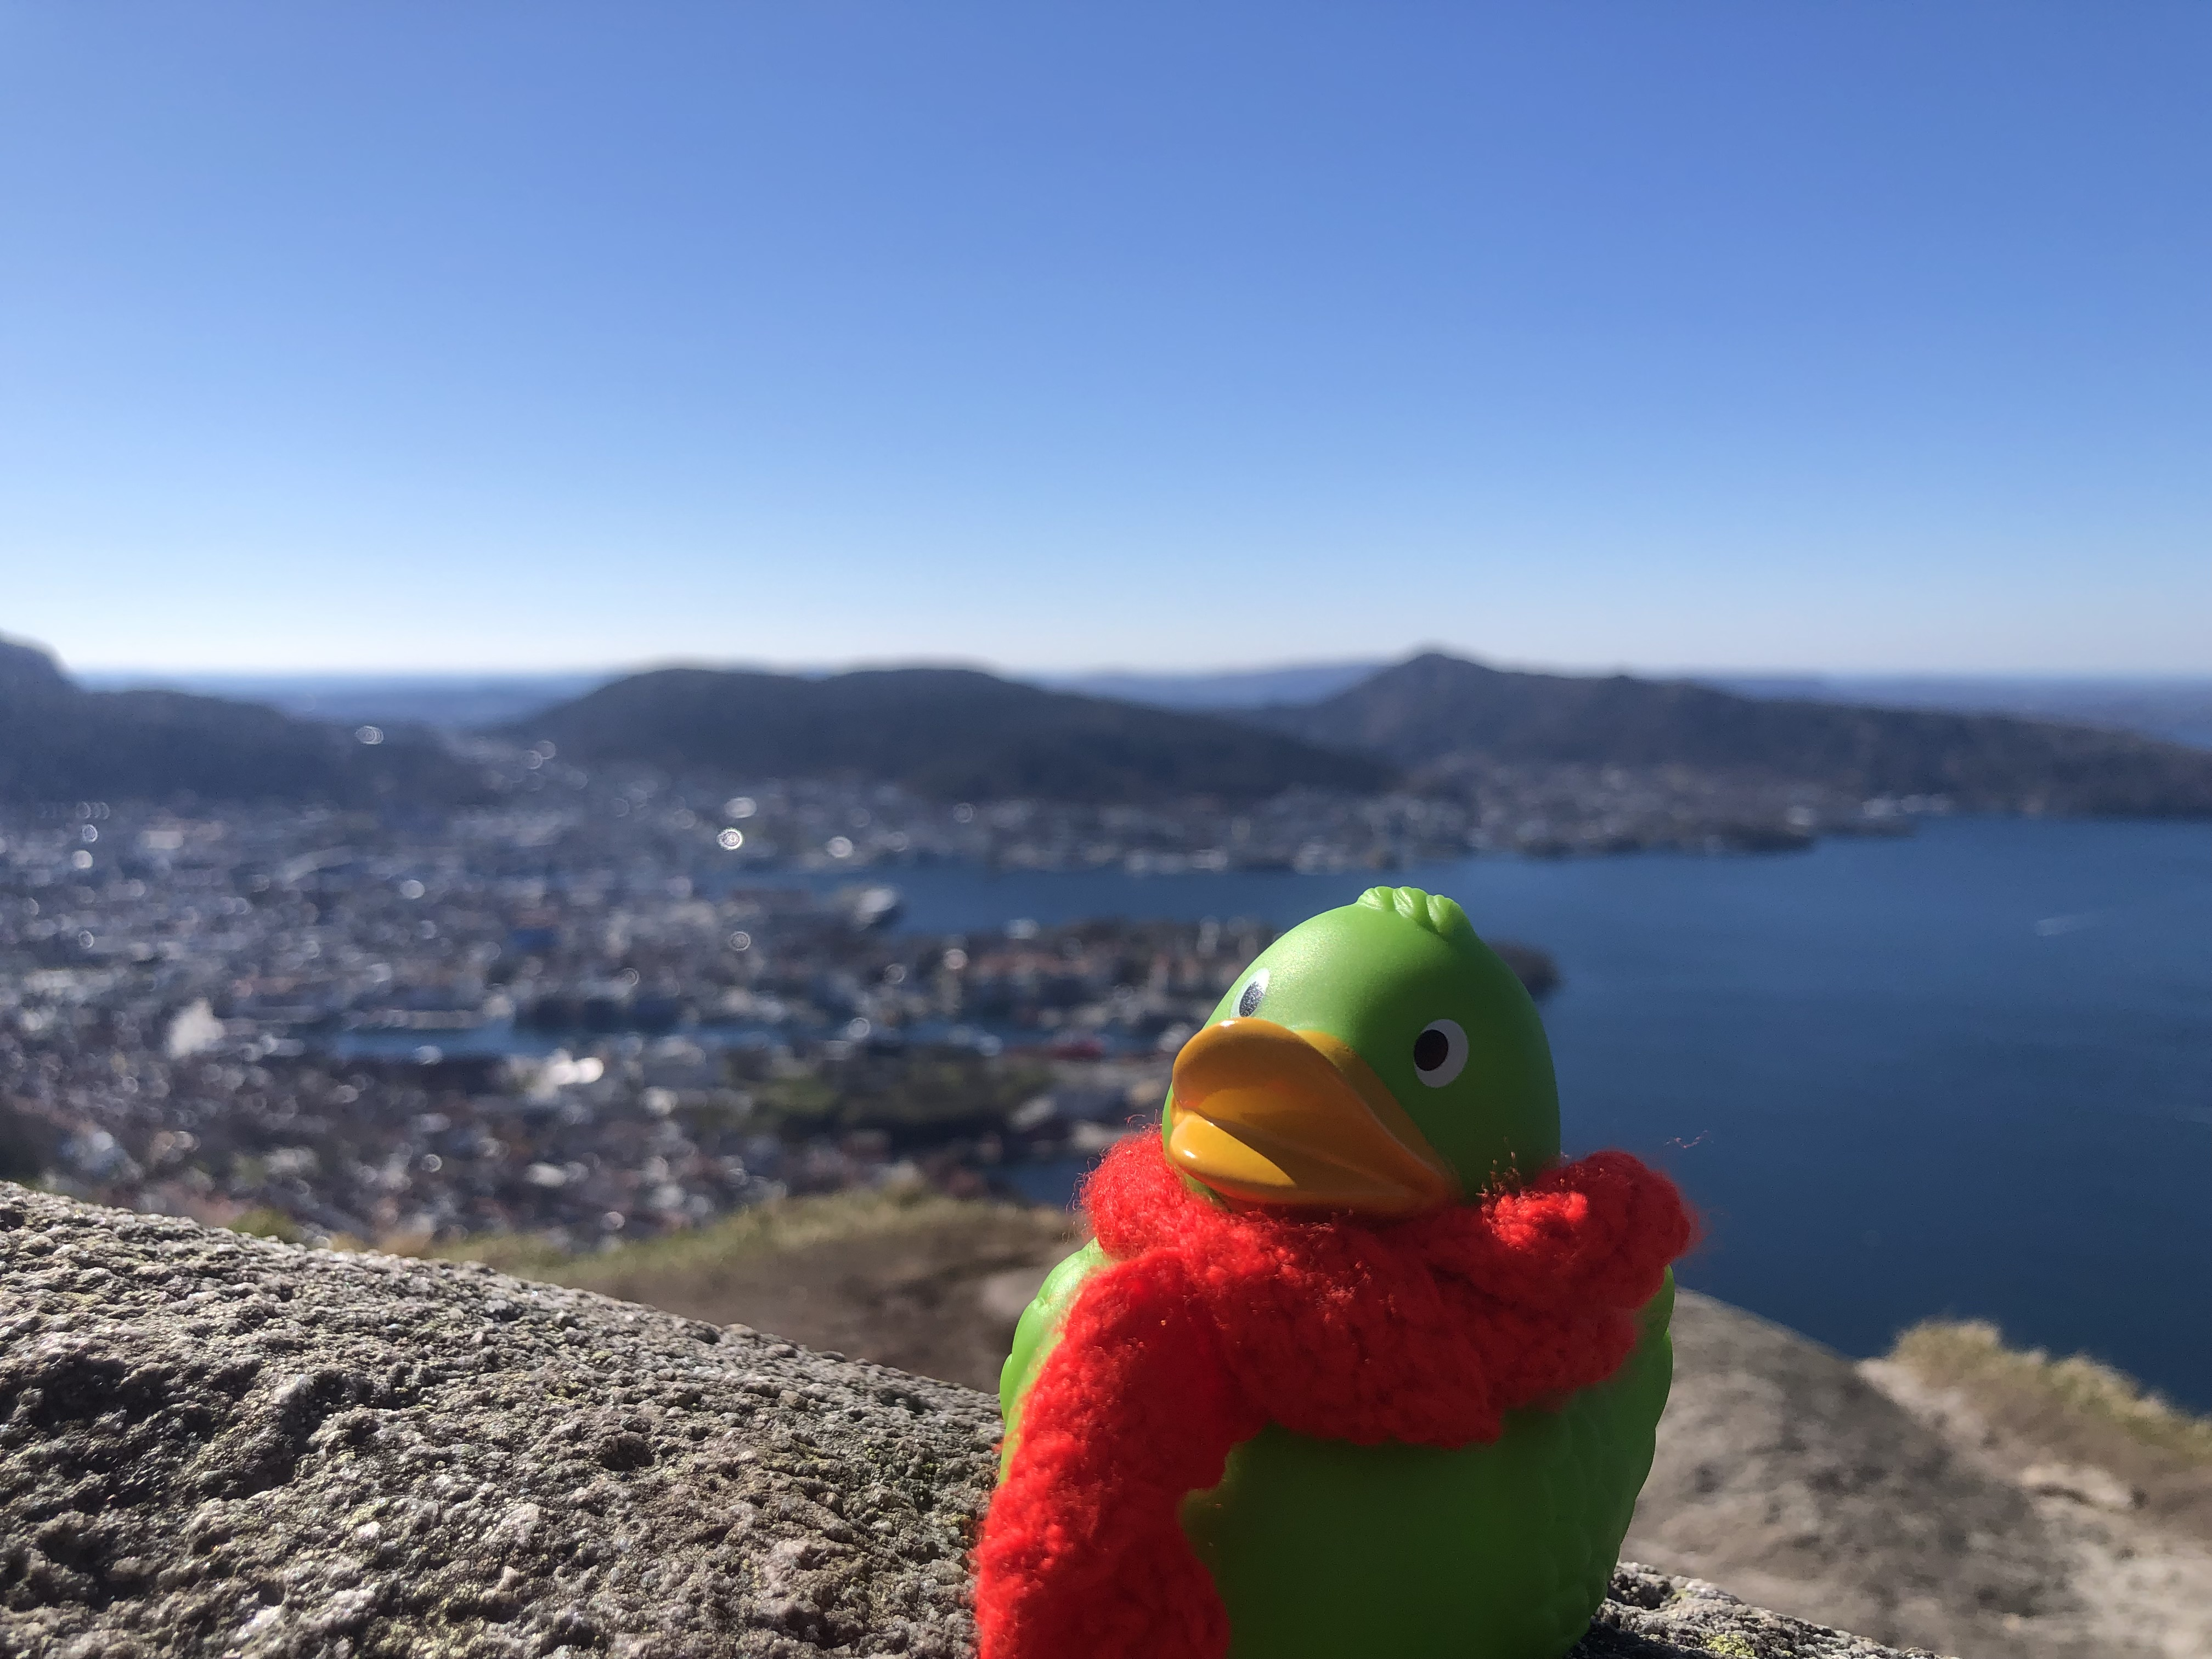
\includegraphics[height = 4.9cm]{images/guillaume1.jpg}
        \caption{Guillaume på Sandviksfjellet}
        \label{fig:guillaume1}
    \end{figure}
\end{frame}

% ===========================

\section{Kryptografi}
\subsection*{Begrep}
\begin{frame}{Symmetrisk og asymmetrisk kryptografi}
\begin{block}{Symmetrisk kryptografi}
\begin{itemize}
\item Det finnes bare \textit{én} nøkkel, som begge personer bruker
\item Brukes for både kryptering og dekryptering
\item Eksempel: Caesar – $f(c) = (c+key) \% mod 26$
\end{itemize}
\end{block}
\pause
\begin{block}{Asymmetrisk kryptografi}
\begin{itemize}
\item Hver person har \textit{to} nøkler: Privat og offentlig
\item Kryptering med offentlig nøkkel av den andre personen
\item Dekryptering med privat nøkkel
\item Eksempel: RSA
\end{itemize}
\end{block}
\end{frame}

\subsection*{RSA}
\begin{frame}{RSA}
\begin{itemize}[<+->]
\item Asymmetrisk kryptering med to nøkler for hver deltaker
\item Kryptering
	\begin{itemize}
	\item Offentlig nøkkel for kryptering
	\item Privat nøkkel for dekryptering
	\end{itemize}
\item Digitale sertifikater/ signaturer
	\begin{itemize}
	\item Privat nøkkel for signering
	\item Offentlig nøkkel for verifisering
	\end{itemize}
\end{itemize}
\end{frame}


\begin{frame}{}
\begin{table}
\begin{tabular}{l|l}
Instruksjon & Eksempel\\ \hline
Velg to primtall $p$, $q$ & $p=7, q=13$\\
Regn ut $n=p\cdot q$ & $7\cdot 13=91$\\
Regn ut $\phi(n)=(p-1)\cdot(q-1)$&$\phi(n)=6\cdot12=72$\\
Velg $e$ med $2<e<\phi(n)$ og $gcd(e,\phi(n))=1$&23, $gcd(72,23)=1$\\
Finn $d=e^{-1} (mod\, \phi(n))$ med EEA & $d=23^{-1} (mod\, 72)$\\
\indent\hspace{3mm} Lineærkombinasjon & $-25\cdot 23+8\cdot 72=1$\\
& $a=-25$, $72-25=47$, $d=47$\\
Kryptering av blokk M & $M=42$\\
\indent\hspace{3mm} $C=M^e(mod\, n)$&$42^{23} (mod\, 91)=35$\\
Dekryptering av blokk C & $C=35$\\
\indent\hspace{3mm} $M=C^d(mod\, n)$&$35^{47} (mod\, 91)=42$
\end{tabular}
\caption{Hvordan brukes RSA?}
\end{table}
\end{frame}

\subsection*{Spørretid}
\begin{frame}{Spørsmål?}
    \begin{figure}
        \centering
        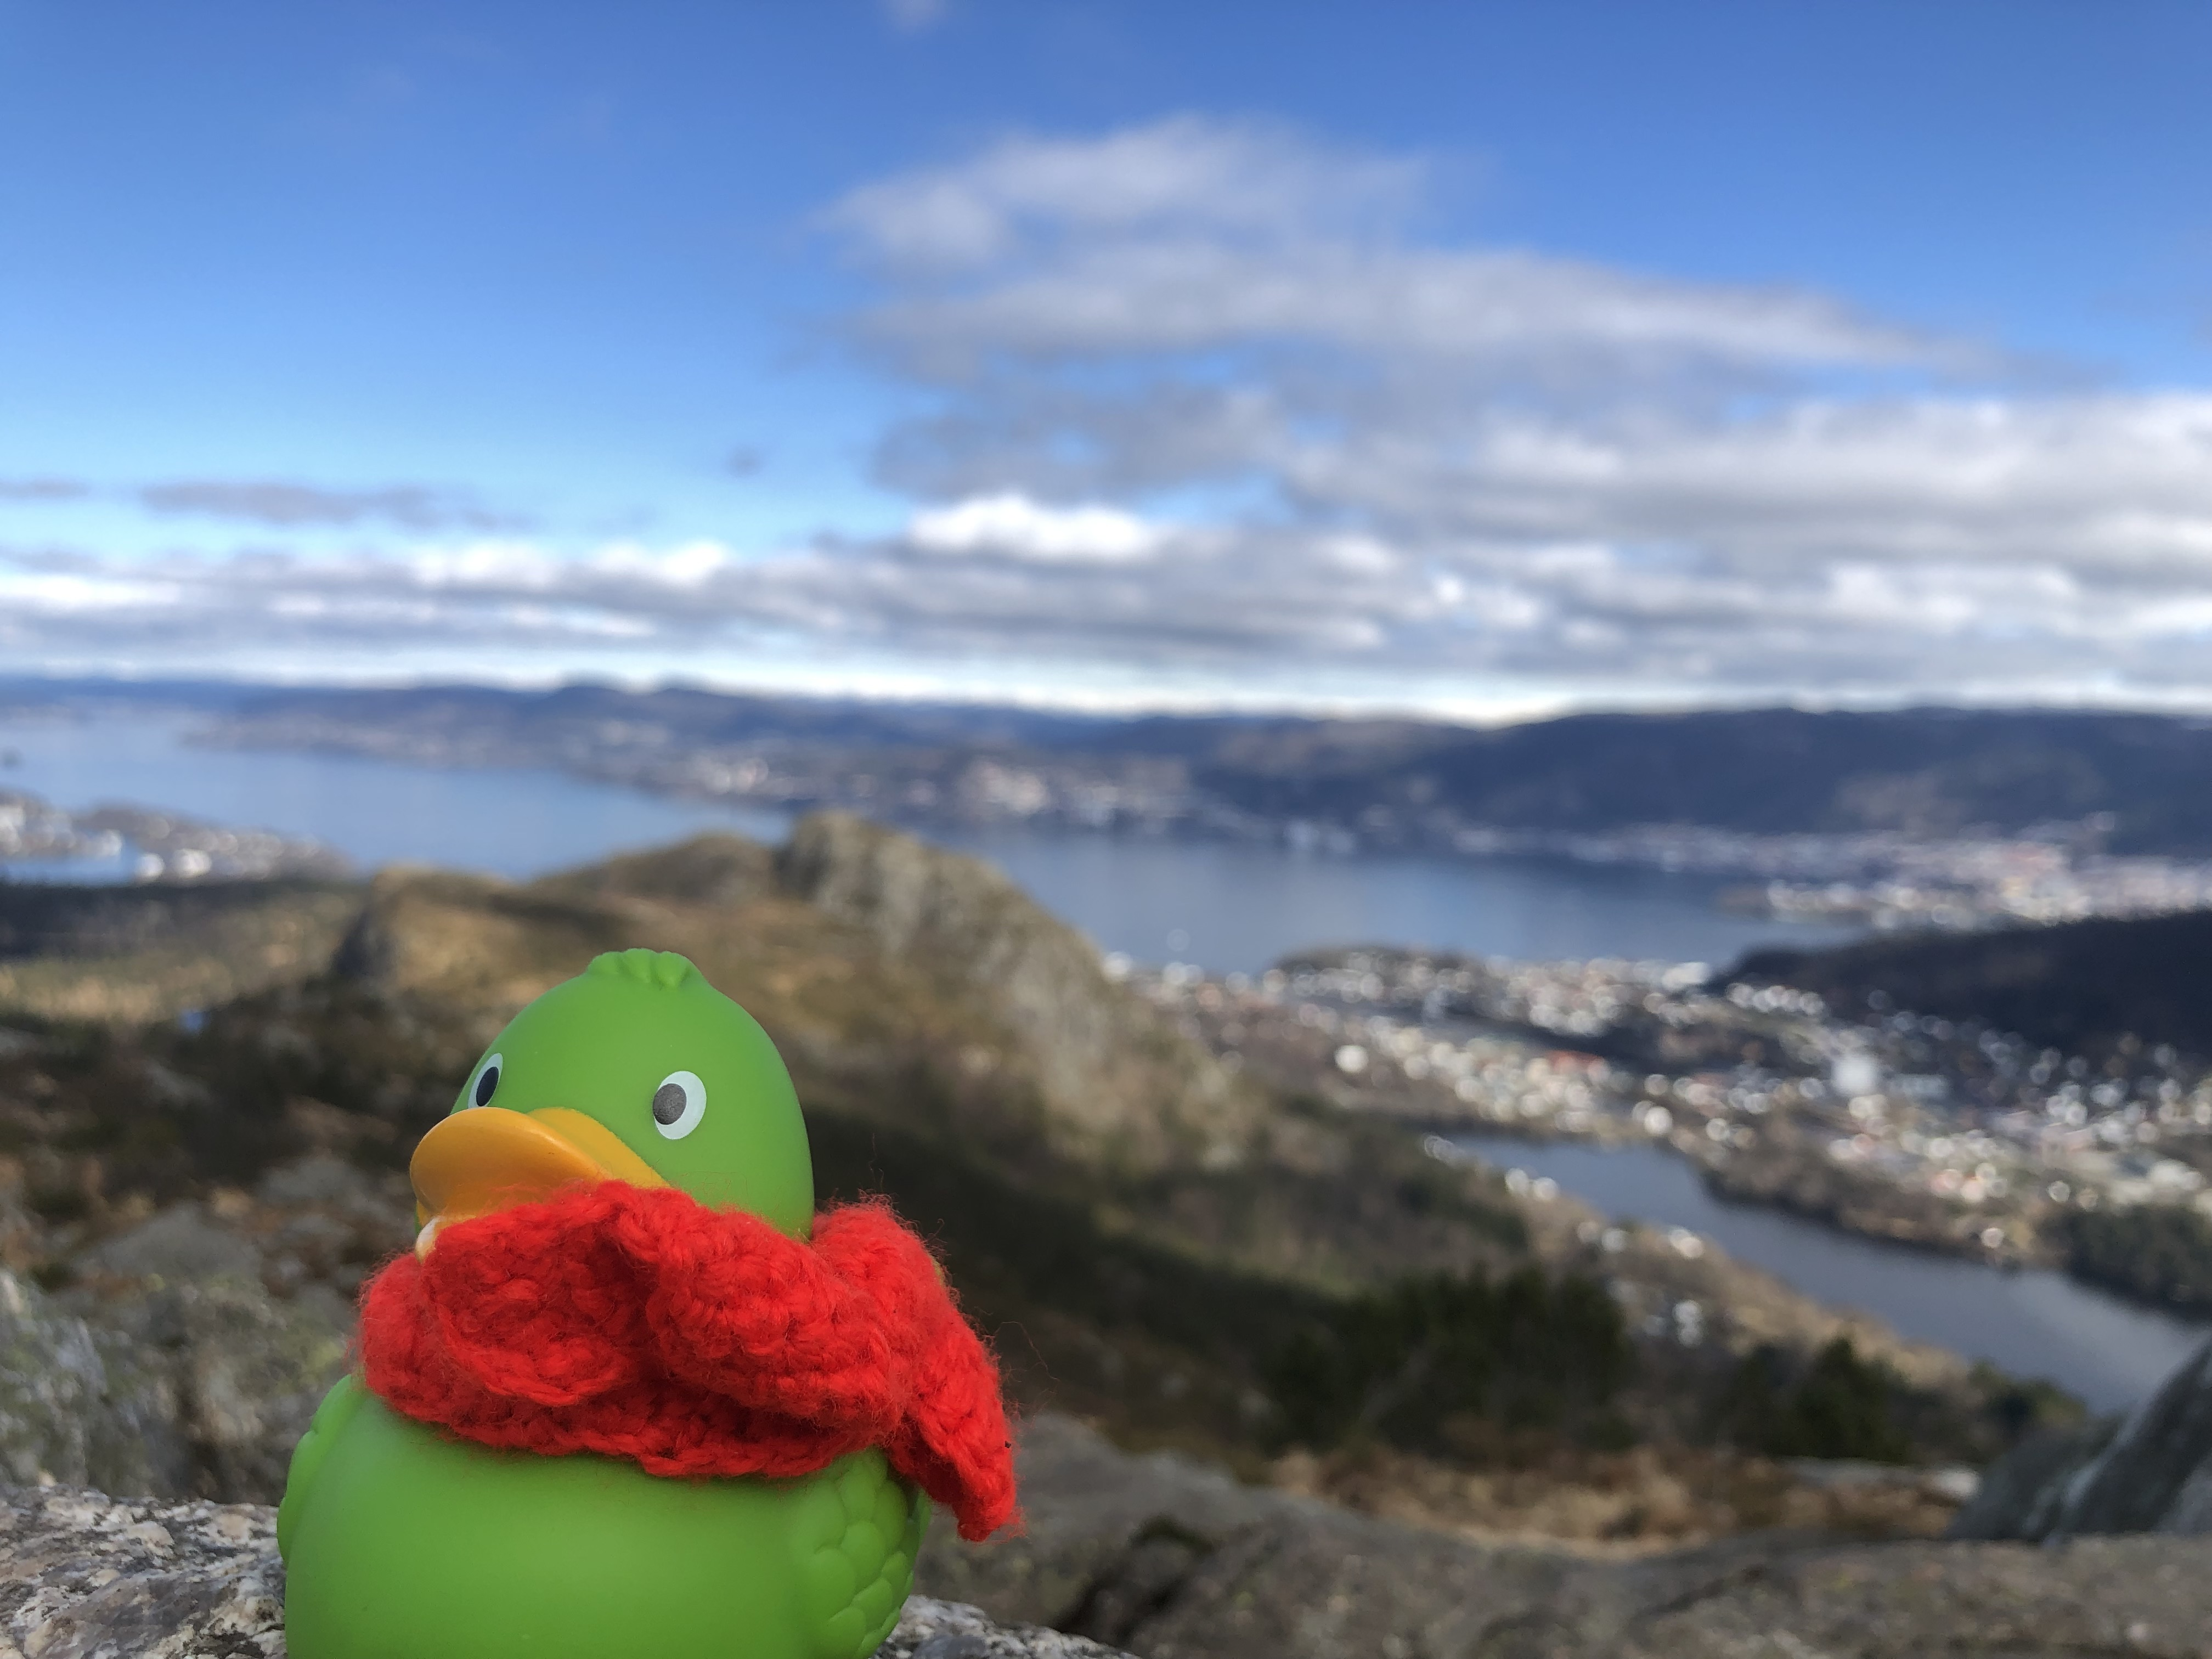
\includegraphics[height = 4.9cm]{images/guillaume8.jpg}
        \caption{Guillaume på Lyderhorn}
        \label{fig:guillaume8}
    \end{figure}
\end{frame}

\section{Stokastisitet}
\subsection{Counting}
\begin{frame}
TODO: Fill with content @Lukas 
Basics of Counting
Pigeonhole Principle
Permutations and Combinations
Binomial conefficients and identities
\end{frame}

\subsection{Sannsynligheter}
\begin{frame}
TODO: Fill with content @Lukas 
Bayes theorem, probabilitiy theory
discrete probability
expected value and variance
\end{frame}




\section{Grafer}
\subsection*{Begrep}
\begin{frame}
    \begin{block}{Graf $G(V,E)$}
    En Graf $G$ er en tuple med en set av noder $V$ og en set av kanter (edges) $E$
    \end{block}
    \pause

\begin{columns}
    \begin{column}{0.28\textwidth}
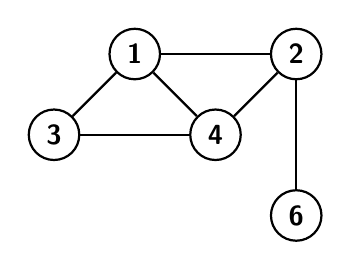
\begin{tikzpicture}[
    node distance=1.45cm, thick,
    main node/.style={circle, draw, font=\sffamily\bfseries}
]
    \node[main node] (1)                    {1};
    \node[main node] (3) [below left  of=1] {3};
    \node[main node] (4) [below right of=1] {4};
    \node[main node] (2) [above right of=4] {2};
    \node[main node] (6) [below right of=4] {6}; % <-4> forces an additional overlay in which node 2 disappears

    \path (1) edge (2)
        (4) edge (2)
        (6) edge (2);
    \path (1) edge (3)
        (4) edge (1);
    \path (3) edge (4);
\end{tikzpicture}
 \end{column}
 \pause
    \begin{column}{0.68\textwidth}
\begin{itemize}[<+->]
    \item Noder: $V={1,2,3,4,6}$
    \item Kanter: $E={(1,2), (1,4), (3,4), (2,4), (2,6), (1,3)}$
    \item Path: Vei fra A til B\\
    Eksempel: $Path(1,6)=(1,2,6)$
    \item Cycle: En path med samme start og slutt\\
    Eksempel: $(1,3,4,1)$, $(1,2,4,3,1)$
    \item Naboer: Set of noder som har en kante til en node\\
    Eksempel: $N(4)={1,2,3}$, $N(6)=2$
    \item Degree: Antall naboer av en node\\
    Eksempel: $deg(4)=3$, $deg(6)=1$
\end{itemize}
 \end{column}
\end{columns}
\end{frame}

\begin{frame}{}
    \begin{columns}
    \begin{column}{0.48\textwidth}
    \begin{figure}
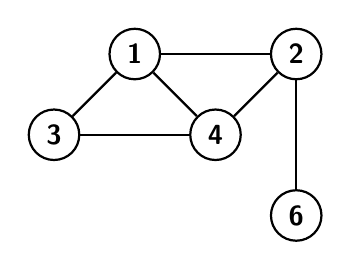
\begin{tikzpicture}[
    node distance=1.45cm, thick,
    main node/.style={circle, draw, font=\sffamily\bfseries}
]
    \node[main node] (1)                    {1};
    \node[main node] (3) [below left  of=1] {3};
    \node[main node] (4) [below right of=1] {4};
    \node[main node] (2) [above right of=4] {2};
    \node[main node] (6) [below right of=4] {6}; % <-4> forces an additional overlay in which node 2 disappears

    \path (1) edge (2)
        (4) edge (2)
        (6) edge (2);
    \path (1) edge (3)
        (4) edge (1);
    \path (3) edge (4);
\end{tikzpicture}
\caption{Urettet graf (undirected)}
\end{figure}
\begin{itemize}
    \item $deg(4) = 3$
\end{itemize}
 \end{column}
 \pause
    \begin{column}{0.48\textwidth}
    \begin{figure}
    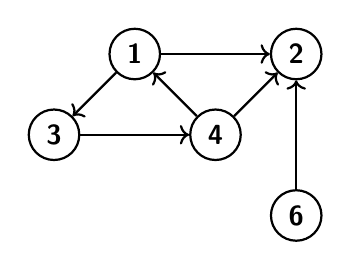
\begin{tikzpicture}[
    node distance=1.45cm, thick,
    main node/.style={circle, draw, font=\sffamily\bfseries}
]
    \node[main node] (1)                    {1};
    \node[main node] (3) [below left  of=1] {3};
    \node[main node] (4) [below right of=1] {4};
    \node[main node] (2) [above right of=4] {2};
    \node[main node] (6) [below right of=4] {6}; % <-4> forces an additional overlay in which node 2 disappears

    \path[->] (1) edge (2)
        (4) edge (2)
        (6) edge (2);
    \path[->] (1) edge (3)
        (4) edge (1);
    \path[->] (3) edge (4);
\end{tikzpicture}
\caption{Rettet graf (directed)}
\end{figure}
\begin{itemize}
    \item $deg^-(4) = 1$ (ingoing)
    \item $deg^+(4) = 2$ (outgoing)
\end{itemize}
 \end{column}
\end{columns}
\end{frame}

\begin{frame}
    \begin{block}{Bipartite graf $G(V,A,B)$}
    Set av nodene er delt i to sets $A,B$ der alle kanter $v\in V$ går fra en node i $A$ til en node i $B$\\
    Grafen kan farges i to farger med ingen to nabonoder i samme farge
    \end{block}

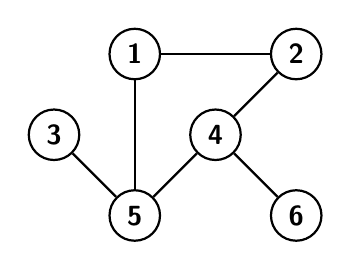
\begin{tikzpicture}[
    node distance=1.45cm, thick,
    main node/.style={circle, draw, font=\sffamily\bfseries}
]
    \node[main node,onslide=<2->{fill=black!40!green}] (1)                    {1};
    \node[main node,onslide=<2->{fill=black!40!green}] (3) [below left  of=1] {3};
    \node[main node,onslide=<2->{fill=black!40!green}] (4) [below right of=1] {4};
    \node[main node,onslide=<2->{fill=black!30!red}] (2) [above right of=4] {2};
    \node[main node,onslide=<2->{fill=black!30!red}] (5) [below right of=3] {5};
    \node[main node,onslide=<2->{fill=black!30!red}] (6) [below right of=4] {6};

    \path (1) edge (2)
        (1) edge (5)
        (3) edge (5)
        (4) edge (2)
        (4) edge (5)
        (4) edge (6);
\end{tikzpicture}
\end{frame}

\subsection*{Representasjon}
\begin{frame}
\begin{center}
\incomplete{5}{1/2,1/3,1/4,1/5,2/4,2/5}
\end{center}
\vspace{-1cm}
\begin{columns}
    \begin{column}{0.48\textwidth}
 \begin{table}[]
\centering
\label{tab:adjmatexample}
\begin{tabular}{r|ccccc}
  & 1 & 2 & 3 & 4 & 5 \\ \hline
1 & 0  & 1  & 1  &  1 & 1  \\
2 & 1  & 0  & 0  &  1 & 1  \\
3 & 1  & 0  & 0  &  0 & 0  \\
4 & 1  & 1  & 0  & 0  & 0  \\
5 & 1  & 1  & 0  & 0  & 0 
\end{tabular}
\caption{Adjacency matrix (directed)}
\end{table}
 \end{column}
    \begin{column}{0.48\textwidth}
\begin{table}[]
\centering
\label{tab:adjlistexample}
\begin{tabular}{r|l}
Node & Neighbours \\ \hline
1   &  {2,3,4,5}          \\
2   &  {1,4,5}          \\
3   &  {1}          \\
4   &  {1,2}          \\
5   &  {1,2}         
\end{tabular}
\caption{Adjacency list (directed)}
\end{table}
 \end{column}
\end{columns}
\end{frame}

\subsection{Trær}
\begin{frame}
\begin{block}{Tre $G(V,E)$}
    Et tre er en \textit{connected}, \textit{undirected} graph der ingen cycles eksisterer.
    \end{block}
    \pause
\begin{block}{Forest $G(V,E)$}
    En mengde av trær som ikke er tilknyttet med hverandre.
    \end{block}
    \pause
\begin{block}{Rooted tre $G(V,E)$}
    Et tre med en root node.
    \end{block}
\end{frame}

\begin{frame}
\begin{columns}
    \begin{column}{0.48\textwidth}
\begin{figure}
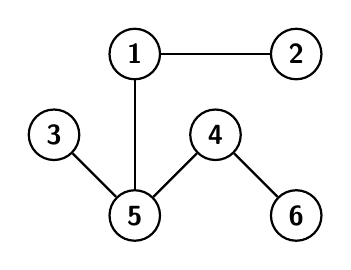
\begin{tikzpicture}[
    node distance=1.45cm, thick,
    main node/.style={circle, draw, font=\sffamily\bfseries}
]
    \node[main node] (1)                    {1};
    \node[main node] (3) [below left  of=1] {3};
    \node[main node] (4) [below right of=1] {4};
    \node[main node] (2) [above right of=4] {2};
    \node[main node] (5) [below right of=3] {5};
    \node[main node] (6) [below right of=4] {6};

    \path (1) edge (2)
        (1) edge (5)
        (3) edge (5)
        (4) edge (5)
        (4) edge (6);
\end{tikzpicture}
\caption{Et tre}
\end{figure}
 \end{column}
 \pause
    \begin{column}{0.48\textwidth}
\begin{figure}
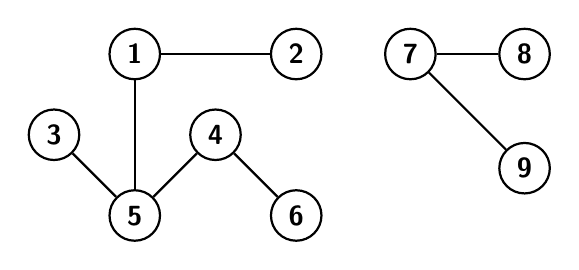
\begin{tikzpicture}[
    node distance=1.45cm, thick,
    main node/.style={circle, draw, font=\sffamily\bfseries}
]
    \node[main node] (1)                    {1};
    \node[main node] (3) [below left  of=1] {3};
    \node[main node] (4) [below right of=1] {4};
    \node[main node] (2) [above right of=4] {2};
    \node[main node] (5) [below right of=3] {5};
    \node[main node] (6) [below right of=4] {6};
    \node[main node] (7) [right of=2] {7};
    \node[main node] (8) [right of=7] {8};
    \node[main node] (9) [below of=8] {9};

    \path (1) edge (2)
        (1) edge (5)
        (3) edge (5)
        (4) edge (5)
        (4) edge (6)
        (7) edge (8)
        (7) edge (9);
\end{tikzpicture}
\caption{En skog (forest)}
\end{figure}
\end{column}
\end{columns}
\end{frame}

\begin{frame}{Rooted trees}
    \begin{block}{binary (m-ary) tre $G(V,E)$}
    Et tre med en root node der alle interne noder har eksakt to (m) barn.
    \end{block}
    \begin{columns}
    \begin{column}{0.48\textwidth}
\begin{figure}
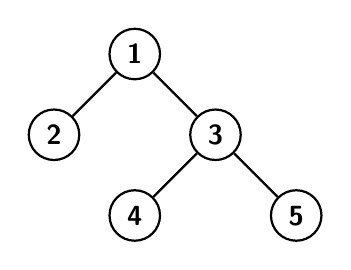
\begin{tikzpicture}[
    node distance=1.45cm, thick,
    main node/.style={circle, draw, font=\sffamily\bfseries}
]
   \node[main node] (1)                    {1};
    \node[main node] (2) [below left  of=1] {2};
    \node[main node] (3) [below right of=1] {3};
    \node[main node] (4) [below left of=3] {4};
    \node[main node] (5) [below right of=3] {5};

    \path (1) edge (2)
        (1) edge (3)
        (3) edge (4)
        (3) edge (5);
\end{tikzpicture}
\caption{binary tre}
\end{figure}
 \end{column}
    \begin{column}{0.48\textwidth}
\begin{figure}
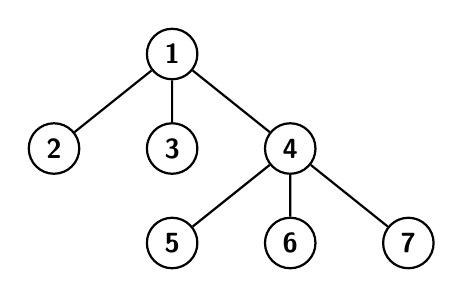
\begin{tikzpicture}[
    node distance=1.45cm, thick,
    main node/.style={circle, draw, font=\sffamily\bfseries},level distance=1.2cm,
  level 1/.style={sibling distance=1.5cm},
  level 2/.style={sibling distance=1.5cm}
]
  \node[main node] {1}
  	child {node[main node] {2}}
    child {node[main node] {3}}
    child {node[main node] {4}
    child {node[main node] {5}}
      child {node[main node] {6}}
    child {node[main node] {7}}
    };
\end{tikzpicture}
\caption{3-ary tre}
\end{figure}
\end{column}
\end{columns}
\end{frame}

\begin{frame}{Egenskaper}
    \begin{itemize}
        \item Et tre med $n$ noder har $n-1$ kanter
    \end{itemize}
   \begin{table}
    \begin{tabular}{l|l|l}
Noder & Interne noder & Leaves \\ \hline
\textbf{$n$} & $i=(n-1)/m$ & $l=((m-1)\cdot n+1)/m$\\
$n=m\cdot i + 1$ & \textbf{$i$} & $l=(m-1)\cdot i+1$\\
$n=(m\cdot l - 1)/(m-1)$ & $i=(l-1)/(m-1)$ & \textbf{$l$}          
\end{tabular}
\caption{Regne ut antall noder for fulle m-ary trær}
\end{table}
\end{frame}

\begin{frame}{Eksempel}
Et kjedebrev starter med en person som sender et brev til fem andre mennesker. Hver person som får et brev sender den enten videre til fem andre eller stopper å sende ting videre.\\
Gå ut ifra at 10.000 personer sender brevet videre og ingen får brevet to ganger.\\
(1) Hvor mange personer fikk et brev?\\
(2) Hvor mange sendte ikke brevet videre?\\\pause
\begin{itemize}
\item Folk som sender videre: Interne noder $i=10000$
\item Folk som ikke sender videre: Leaves $l = (5-1)\cdot 10000 + 1 = 40001$
\item Folk som fikk et brev: Noder $n=5\cdot 10000 + 1 = 50001$
\end{itemize}
\end{frame}

\subsection*{Spørretid}
\begin{frame}{Spørsmål?}
    \begin{figure}
        \centering
        \includegraphics[height = 4.9cm]{images/guillaume9.jpg}
        \caption{Guillaume foran Tvindefossen}
        \label{fig:guillaume9}
    \end{figure}
\end{frame}

\subsection{Algoritmer}
%\begin{frame}{Preorder Traversal}
%TODO: Fill with content @Lukas 
%\end{frame}
%
%\begin{frame}{Postorder Traversal}
%TODO: Fill with content @Lukas 
%\end{frame}
%
%\begin{frame}{Inorder Traversal}
%TODO: Fill with content @Lukas 
%\end{frame}

\begin{frame}{Spanning Trees}
	\begin{block}{Spanning Trees}
    Et Spanning Tree for en graf er et tree som besøker alle noder, men ikke lager cycles.
    \end{block}
    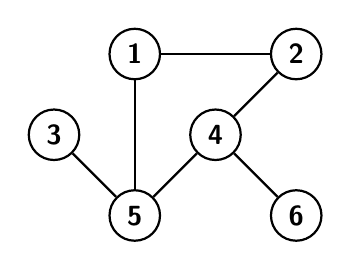
\begin{tikzpicture}[
    node distance=1.45cm, thick,
    main node/.style={circle, draw, font=\sffamily\bfseries}
]
    \node[main node] (1)                    {1};
    \node[main node] (3) [below left  of=1] {3};
    \node[main node] (4) [below right of=1] {4};
    \node[main node] (2) [above right of=4] {2};
    \node[main node] (5) [below right of=3] {5};
    \node[main node] (6) [below right of=4] {6};

    \path (1) edge (2)
        (1) edge (5)
        (3) edge (5)
        (4) edge (2)
        (4) edge (5)
        (4) edge (6);
\end{tikzpicture}
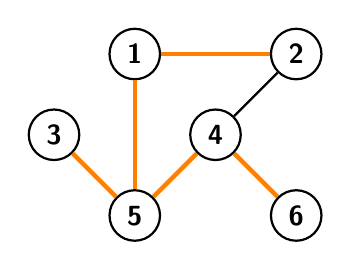
\begin{tikzpicture}[
    node distance=1.45cm, thick,
    main node/.style={circle, draw, font=\sffamily\bfseries}
]
    \node[main node] (1)                    {1};
    \node[main node] (3) [below left  of=1] {3};
    \node[main node] (4) [below right of=1] {4};
    \node[main node] (2) [above right of=4] {2};
    \node[main node] (5) [below right of=3] {5};
    \node[main node] (6) [below right of=4] {6};

    \path (1) edge[properties] (2)
        (1) edge[properties] (5)
        (3) edge[properties] (5)
        (4) edge (2)
        (4) edge[properties] (5)
        (4) edge[properties] (6);
\end{tikzpicture}
\end{frame}

\begin{frame}{Algoritmer for Spanning Trees}
Finne \textit{en} Spanning Tree
\begin{itemize}
\item Breadth-first search (BFS)
\item Depth-first search (DFS)
\end{itemize}
\hspace{1cm}

\noindent Finne \textit{en} Minimum Spanning Tree
\begin{itemize}
\item Prims algoritme
\item Kruskals algoritme
\end{itemize}
\end{frame}

\begin{frame}{BFS og DFS}
\begin{itemize}
\item Begge to går gjennom grafen fra en startnode
\item I hver runde går man videre til naboene til en node
\item Forskjell: BFS bruker kø, DFS stack
\item BFS: Rekkefølgen noder blir markert er rekkefølgen man går gjennom grafen
\item $\rightarrow$ Bredden blir utforsket før
\item DFS: Første noder som blir markiert er siste man ser på
\item $\rightarrow$ Algoritmen søker dypt først
\end{itemize}
\end{frame}

\begin{frame}[fragile]{Breadth-first search (BFS)}
\begin{minted}{python}
def bfs(graph):
   visited = [node] # alle besøkte noder
   queue = [node]   # køen
	
   while queue:     # så lenge noder er igjen
      m = queue.pop(0) # neste node 
      print(f"Visited: {m}")
      for neighbour in graph.neighbours(m): # gå gjennom naboer
         if neighbour not in visited:       # hvis ikke sett før
            visited += neighbour            # add til visited og kø
            queue += neighbour
\end{minted}
\end{frame}

\begin{frame}{Eksempel BFS}
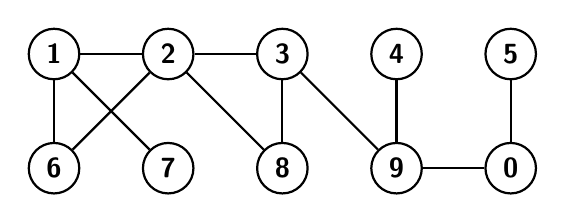
\begin{tikzpicture}[
    node distance=1.45cm, thick,
    main node/.style={circle, draw, font=\sffamily\bfseries}
]
    \node[main node] (1) [onslide=<1->{fill=black!30!red}]                   {1};
    \node[main node] (2) [right of =1,onslide=<2->{fill=black!30!red}] {2};
    \node[main node] (3) [right of =2,onslide=<3->{fill=black!30!red}] {3};
    \node[main node] (4) [right of =3,onslide=<5->{fill=black!30!red}] {4};
    \node[main node] (5) [right of =4,onslide=<6->{fill=black!30!red}] {5};
    \node[main node] (6) [below of =1,onslide=<2->{fill=black!30!red}] {6};
    \node[main node] (7) [right of =6,onslide=<2->{fill=black!30!red}] {7};
    \node[main node] (8) [right of =7,onslide=<3->{fill=black!30!red}] {8};
    \node[main node] (9) [right of =8,onslide=<4->{fill=black!30!red}] {9};
    \node[main node] (0) [right of =9,onslide=<5->{fill=black!30!red}] {0};

    \path (1) edge[onslide=<1->{propertiesBlue},onslide=<2->{propertiesRed}] (2)
        (1) edge[onslide=<1->{propertiesBlue},onslide=<2->{propertiesRed}] (6)
        (1) edge[onslide=<1->{propertiesBlue},onslide=<2->{propertiesRed}] (7)
        (2) edge[onslide=<2->{propertiesBlue},onslide=<3->{propertiesRed}] (3)
        (2) edge[onslide=<2->{propertiesBlue},onslide=<3->{propertiesRed}] (8)
        (3) edge (8)
		(3) edge[onslide=<3->{propertiesBlue},onslide=<4->{propertiesRed}] (9)
        (4) edge[onslide=<4->{propertiesBlue},onslide=<5->{propertiesRed}] (9)
        (9) edge[onslide=<4->{propertiesBlue},onslide=<5->{propertiesRed}] (0)
        (0) edge[onslide=<5->{propertiesBlue},onslide=<6->{propertiesRed}] (5)
        (2) edge (6);
\end{tikzpicture}
\medskip

\only<1>{
	Queue: 2 6 7
}
\only<2>{
	Queue: \cancel{2} \cancel{6} \cancel{7} 3 8
}
\only<3>{
	Queue: \cancel{2} \cancel{6} \cancel{7} \cancel{3} \cancel{8} 9
}
\only<4>{
	Queue: \cancel{2} \cancel{6} \cancel{7} \cancel{3} \cancel{8} \cancel{9} 4 0
}
\only<5>{
	Queue: \cancel{2} \cancel{6} \cancel{7} \cancel{3} \cancel{8} \cancel{9} \cancel{4} \cancel{0} 5
}
\only<6>{
	Queue: \cancel{2} \cancel{6} \cancel{7} \cancel{3} \cancel{8} \cancel{9} \cancel{4} \cancel{0} \cancel{5}
}
\end{frame}

\begin{frame}[fragile]{Depth-first search (DFS)}
\begin{minted}{python}
visited = []	# alle besøkte noder

def dfs(visited, graph, node):
   if node not in visited:      # hvis noden ikke er besøkt
      print(f"Visited: {node}") # markere som besøkt
      visited += node
      
      for neighbour in graph.neighbours(node): # gå gjennom naboer
         dfs(visited, graph, neighbour)        # rekursiv call
\end{minted}
\end{frame}

\begin{frame}{Eksempel DFS}
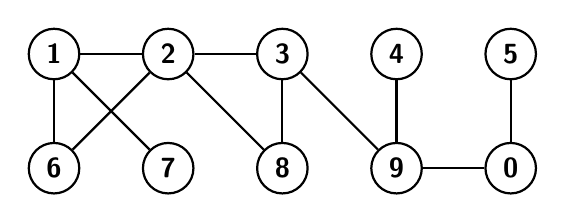
\begin{tikzpicture}[
    node distance=1.45cm, thick,
    main node/.style={circle, draw, font=\sffamily\bfseries}
]
    \node[main node] (1) [onslide=<1->{fill=black!30!red}]                   {1};
    \node[main node] (2) [right of =1,onslide=<3->{fill=black!30!red}] {2};
    \node[main node] (3) [right of =2,onslide=<4->{fill=black!30!red}] {3};
    \node[main node] (4) [right of =3,onslide=<7->{fill=black!30!red}] {4};
    \node[main node] (5) [right of =4,onslide=<9->{fill=black!30!red}] {5};
    \node[main node] (6) [below of =1,onslide=<11->{fill=black!30!red}] {6};
    \node[main node] (7) [right of =6,onslide=<12->{fill=black!30!red}] {7};
    \node[main node] (8) [right of =7,onslide=<5->{fill=black!30!red}] {8};
    \node[main node] (9) [right of =8,onslide=<6->{fill=black!30!red}] {9};
    \node[main node] (0) [right of =9,onslide=<8->{fill=black!30!red}] {0};

    \path (1) edge[onslide=<2->{propertiesBlue},onslide=<3->{propertiesRed}] (2)
        (1) edge[onslide=<2-11>{propertiesBlue}] (6)
        (1) edge[onslide=<2-11>{propertiesBlue},onslide=<12->{propertiesRed}] (7)
        (2) edge[onslide=<3-3>{propertiesBlue},onslide=<4->{propertiesRed}] (3)
        (2) edge[onslide=<3-9>{propertiesBlue}] (8)
        (3) edge[onslide=<4-5>{propertiesBlue},onslide=<5->{propertiesRed}] (8)
		(3) edge[onslide=<4-5>{propertiesBlue},onslide=<6->{propertiesRed}] (9)
        (4) edge[onslide=<6-6>{propertiesBlue},onslide=<7->{propertiesRed}] (9)
        (9) edge[onslide=<6-7>{propertiesBlue},onslide=<8->{propertiesRed}] (0)
        (0) edge[,onslide=<8-8>{propertiesBlue},onslide=<9->{propertiesRed}] (5)
        (2) edge[onslide=<3-10>{propertiesBlue},onslide=<11->{propertiesRed}] (6);
\end{tikzpicture}
\medskip

\only<1>{
	Stack: 
}
\only<2>{
	Stack: 7 6 2
}
\only<3>{
	Stack: 7 6 \cancel{2} 6 8 3
}
\only<4>{
	Stack: 7 6 \cancel{2} 6 8 \cancel{3} 9 8
}
\only<5>{
	Stack: 7 6 \cancel{2} 6 8 \cancel{3} 9 \cancel{8}
}
\only<6>{
	Stack: 7 6 \cancel{2} 6 8 \cancel{3} \cancel{9} \cancel{8} 0 4
}
\only<7>{
	Stack: 7 6 \cancel{2} 6 8 \cancel{3} \cancel{9} \cancel{8} 0 \cancel{4}
}
\only<8>{
	Stack: 7 6 \cancel{2} 6 8 \cancel{3} \cancel{9} \cancel{8} \cancel{0} \cancel{4} 5
}
\only<9>{
	Stack: 7 6 \cancel{2} 6 8 \cancel{3} \cancel{9} \cancel{8} \cancel{0} \cancel{4} \cancel{5}
}
\only<10>{
	Stack: 7 6 \cancel{2} 6 \cancel{8} \cancel{3} \cancel{9} \cancel{8} \cancel{0} \cancel{4} \cancel{5}
}
\only<11>{
	Stack: 7 6 \cancel{2} \cancel{6} \cancel{8} \cancel{3} \cancel{9} \cancel{8} \cancel{0} \cancel{4} \cancel{5}
}
\only<12>{
	Stack: \cancel{7} \cancel{6} \cancel{2} \cancel{6} \cancel{8} \cancel{3} \cancel{9} \cancel{8} \cancel{0} \cancel{4} \cancel{5}
}
\end{frame}

\begin{frame}{Minimum Spanning Trees}
\begin{block}{Minimum Spanning Trees}
    Et Minimum Spanning Tree for en graf er en Spanning Tree der summen av vektene (weights) er minimal.
    \end{block}
\begin{block}{Kruskals algoritme}
1. Sorter alle kanter etter sine vekter\\
2. Velg kanten med minst vekt som ikke ble valgt før. Hvis det nå blir en syklus, ignorer kanten. Hvis ikke, legg kanten til treet.\\
3. Repeter (2) så lenge til det er (n-1) kanter / alle noder er knyttet sammen.\\
\end{block}
\end{frame}


\begin{frame}{Eksempel Kruskal}
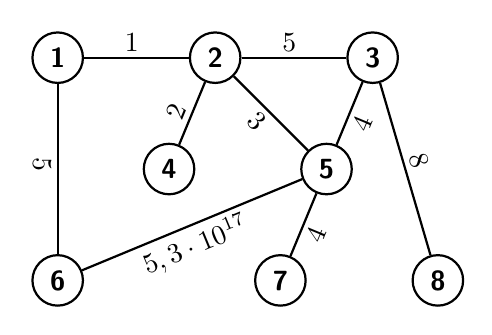
\begin{tikzpicture}[
    node distance=2cm, thick,
    main node/.style={circle, draw, font=\sffamily\bfseries},el/.style = {inner sep=2pt, align=left, sloped},
every label/.append style = {font=\tiny}
]
    \node[main node] (1) [onslide=<3->{fill=black!30!red}] {1};
    \node[main node] (2) [onslide=<3->{fill=black!30!red},right of =1] {2};
    \node[main node] (3) [onslide=<9->{fill=black!30!red},right of =2] {3};
    \node[main node] (4) [onslide=<5->{fill=black!30!red},below right of =1] {4};
    \node[main node] (5) [onslide=<7->{fill=black!30!red},below right of =2] {5};
    \node[main node] (6) [onslide=<15->{fill=black!30!red},below left of =4] {6};
    \node[main node] (7) [onslide=<11->{fill=black!30!red},below right of =4] {7};
    \node[main node] (8) [onslide=<17->{fill=black!30!red},below right of =5] {8};
    
    \path (1)  edge[onslide=<2-2>{propertiesBlue},onslide=<3->{propertiesRed}] node[el,above]  {1}  (2)
     (2)  edge[onslide=<12-12>{propertiesBlue},onslide=<13->{propertiesGrey}] node[el,above]  {5}  (3)
     (1)  edge[onslide=<14-14>{propertiesBlue},onslide=<15->{propertiesRed}] node[el,below]  {5}  (6)
     (2)  edge[onslide=<4-4>{propertiesBlue},onslide=<5->{propertiesRed}] node[el,above]  {2}  (4)
     (2)  edge[onslide=<6-6>{propertiesBlue},onslide=<7->{propertiesRed}] node[el,below]  {3}  (5)
     (3)  edge[onslide=<8-8>{propertiesBlue},onslide=<9->{propertiesRed}] node[el,below]  {4}  (5)
     (5)  edge[onslide=<10-10>{propertiesBlue},onslide=<11->{propertiesRed}] node[el,below]  {4}  (7)
     (3)  edge[onslide=<16-16>{propertiesBlue},onslide=<17->{propertiesRed}] node[el,above]  {8}  (8)
     (6)  edge[onslide=<18->{propertiesGrey}] node[el,below]  {$5,3\cdot 10^{17}$}  (5);
\end{tikzpicture}

\end{frame}

%\section*{Slutt}
\begin{frame}
\begin{center}
\begin{Large}
\textbf{Lykke til på eksamen!\\[5mm]
Takk for oss :)}

\end{Large}
\end{center}  
\end{frame}
\end{document}